\documentclass[10pt,a4paper,ngerman]{scrartcl}
\usepackage[utf8]{inputenc}
\usepackage[ngerman]{babel}
\usepackage[T1]{fontenc}
\usepackage{amsmath}
\usepackage{amsfonts}
\usepackage{amssymb}
\usepackage{makeidx}
\usepackage{graphicx}
\usepackage{epstopdf}
\usepackage[onehalfspacing]{setspace}
\usepackage{array}
\usepackage{upgreek}
\usepackage{float}
\usepackage{csquotes}
\usepackage{chemformula}
\usepackage{chemgreek}
\usepackage{chemmacros}
\chemsetup{modules=all}
\usepackage{tikz}
\usepackage{siunitx}
\sisetup{locale = DE,per-mode = symbol}
\sisetup{output-decimal-marker = {.}}
\usepackage{esvect}
\usepackage{geometry}
\usepackage{pdfpages}
\usepackage[font=small]{caption}
%\usepackage[version=4]{mhchem}
\usepackage[backend=biber, style=chem-angew]{biblatex}
\addbibresource{Visc.bib}
\usepackage{tabularx, booktabs, multirow}
\usepackage[pdfborder={0 0 0}]{hyperref}
\usepackage{scrlayer-scrpage}%Header für die KOMA-script -Klasse
%\usepackage{hyperref}
\usepackage{pgfplots}
\usepackage{textgreek}


\newcommand{\tildenu}{{\fontencoding{LGR}\selectfont\accperispomeni\textnu}}
\captionsetup{format=plain}
\chemsetup[phases]{pos=sub}
\chemsetup[redox]{pos=top}
\chemsetup[redox]{align=center}
%\chemsetup[redox]{explicit-sign=true}
%\chemsetup[redox]{roman=false}
\newcommand{\celsius}{^{\circ}\mathrm{C}}
\parindent0pt
\sloppy
\DeclareChemPhase{\s}{s}
\DeclareChemPhase{\l}{l}
\DeclareChemPhase{\g}{g}
\renewcaptionname{ngerman}{\figurename}{Abb.}
\renewcaptionname{ngerman}{\tablename}{Tab.}
\geometry{bottom=100pt} \geometry{top=80pt}
\newcommand{\m}{\mathrm{m}}
\newcommand{\K}{\mathrm{K}}
\newcommand{\J}{\mathrm{J}}
\newcommand{\gr}{\mathrm{g}}
\newcommand{\kg}{\mathrm{kg}}
\newcommand{\mol}{\mathrm{mol}}
\newcommand{\Pa}{\mathrm{Pa}}
\newcommand{\ad}{\mathrm{ad}}
\newcommand{\de}{\mathrm{de}}
\newcommand{\gmol}{\mathrm{\frac{g}{mol}}}
\newcommand{\JKmol}{\mathrm{\frac{J}{K \cdot mol}}}
\newcommand{\kgmss}{\mathrm{\frac{kg}{m \cdot s^2}}}
\newcommand{\loge}{\mathrm{ln}}


\begin{document}
\begin{titlepage}
	\vspace*{2,5cm}
	\begin{center}
		\begin{LARGE}
			\textbf{Polymer Chemie}\\
			\textbf{Viscometry}\\
		\end{LARGE}
		\vspace{1cm}
		\textbf{Universität Stuttgart}\\
		\vspace*{1,5cm}
		\begin{tabular}{lp{7,5cm}l}
			Author 1:     &Laurens Viehoff\\
            Author 2:     &Felix Roth\\   
			E-Mail 1:      &st183688@stud.uni-stuttgart.de\\
            E-Mail 2:      &st188157@stud.uni-stuttgart.de  \\
			Student-ID 1: & 3676761   \\ 
            Student-ID 2: & 3711192 \\ \\
			Assistentin:  & Yanzhe Huang  \\ \\ 
		\end{tabular}
	\end{center}

    
\end{titlepage}
\thispagestyle{empty}
\renewcommand{\thepage}{\arabic{page}}
\newpage
\tableofcontents
\setcounter{page}{1}
\renewcommand{\thepage}{\arabic{page}}
\newpage



\section{Theory}	

	\subsection{Viscosity}

		In a flowing liquid the brutto-fluid-flowing-peed is reversed proporional to the viscosity. 
		This is because at the wall of the pipe or flask there is a flowgradient. 
		This gradient can be described by many different fast flowing layers also shown in scheme \ref{rohr}.

			\begin{figure}[H]
				\centering
				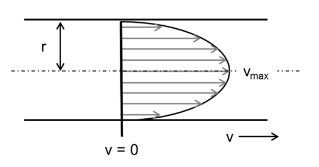
\includegraphics{Bilder/Rohr.png}
				\caption{The picture shows a liquid flöowing through a pipe with the simplyfication of the fluid layers. $r$- is the capillaryradius and v is the flowspeed. \cite{polyskript}}
				\label{rohr}
			\end{figure}

		
		

		Viscosity in polymers is influenced by 5 key factors.
		The first being the volume of the polymer coil, the bigger the coil the more viscouse the fluid gets.
		This is due to the frictional forces.\\
		The second influence is the chemical structure of the polymer, different functional groups mean different intermolecular forces.
		For example if the side chain has a substituent which can make H-Bonds the viscosity gets lower.
		In total it can be stated, the stronger the intramolecular forces the lower the viscosity.\\

		The third one is the influence of the solvent. Different solvents interact with polymers to varying degrees. If, for example, the interaction is very strong, 
		a large amount of solvent will condense onto the polymer and become solvated. However, this also increases the hydrodynamic volume, making the sample more 
		viscous. The increase in viscosity is due to the fact that, with a higher volume, the particles occupy more surface area, thereby reducing the viscosity 
		gradient of the solution. \\

		The fourth is the influence of the concentration. This means with different concentration the viscosity changes.
		This is because the proportion of small solvent particles decreases, thereby inhibiting diffusion. This occurs because the polymer coils are very large and, 
		given limited space, have little freedom of movement and become rigid. In addition, the solution increasingly takes on the properties of the pure polymer, which 
		are usually viscous to solid. \\

		The last but not least influence is the temperature. The viscosity changes with different temperatures, because the movement of the molecules changes.
		If, for example, the temperature rises, the energy of the interactions may be exceeded, causing them to break. Once these interactions are broken, the polymer 
		becomes more freely mobile and no longer resembles a rigid coil. Consequently, the viscosity decreases.\cite{polyskript}\\

	\subsection{From viscosity to $M_\eta$}

		The viscosity is defined after Hagen-Poiseuille by following equation:

			\begin{equation}
				\eta = \frac{\pi\cdot r^4 \cdot t \cdot \Delta p}{8\cdot l \cdot V}
				\label{viscosity}
			\end{equation}

		In which the $\Delta p$ is defindet as:
			
			\begin{equation}
				\Delta p = \rho \cdot g \cdot h
			\end{equation}

		In these equations $r$ is the capillaryradius, $t$ is the time the polymer needs to flow through the capillary,
		$\Delta p$ is the pressure difference in the capillary, $l$ is the lenght of the capillary, $V$ is the Volume, 
		$\rho$ is the density of the solution and $h$ is the height of the measured part.

		After analyzing different polymers four different types of Viscosities could be determined. With $c$ for concentration of the polymersolution.

			\begin{eqnarray}
				\eta_\text{rel} =& \frac{\eta}{\eta_0}\\
				\eta_\text{sp} =& \eta_\text{rel} - 1^\\ 
				\eta_\text{red} =& \frac{\eta_\text{sp}}{c}\\ 
				\eta_\text{} =& \frac{\ln \eta_\text{rel}}{c}
			\end{eqnarray}
		
		 
		If equation \eqref{viscosity} is taken into account $\eta_\text{sp}$ is changed to:
		
			\begin{equation}
				\eta_\text{sp} = \frac{t\rho - t_0\rho_0}{t_0\rho_0}
			\end{equation}

		And because of the low concentration the density of the solution is almost equal to the density of the solvent.
		Therefore the equation can be simplyfied.
			
			\begin{equation}
				\label{spezifischeViskosität}
				\eta_\text{sp} \approx \frac{t-t_0}{t_0}
			\end{equation}

	\newpage

		To get the viscousmiddeled molecular volume the Staudinger-index is used, and it is connected via the 
		Marc-Houwink-Equation. 
		
			\begin{equation}
				\label{ViskosiätsnummerundMolekulargewicht}
				[\eta] = K \cdot \bar{M_\eta^a}
			\end{equation}

		This relationship between the Staudinger index and molecular weight is the subject of the investigation. This is because the Staudinger-index describes the 
		viscosity of a solution at infinite dilution, i.e. a polymer chain. Depending on the volume, this chain has a varying degree of influence on viscosity. As this 
		volume is related to chain length, solvent and temperature, there are also the parameters $K$ and $a$, which take the solvent and temperature into account. The 
		molecular weight can therefore be determined using the Staudinger index.\\
		The viscosity at infinite dilution, i.e. the Staudinger-index, is calculated by extrapolating the reduced viscosity to a concentration of $c = 0$.

			\begin{equation}
				[\eta] = \lim_{c\rightarrow0} (\eta_\text{red}) =\lim_{c\rightarrow0} \left( \frac{\eta_\text{sp}}{c}\right) 
			\end{equation}
		

		So by extrapolating $\eta_\text{red}$, $[\eta]$ can be determined and from that $\bar{M_\eta}$ can be determined. \cite{polyskript}


\section{Experimental}

		The five different polymer solutions were already prepared and ready to use. 
		One pure Toluene solution and four polymer solutions with different concentrations. 
		The concentrations being \SI{1.25}{\frac{g}{l}}, \SI{2.5}{\frac{g}{l}}, \SI{5}{\frac{g}{l}} and \SI{10}{\frac{g}{l}}.
		All of these five solutions were analyzed with a Viscosimeter.

\section{Results}

		In order to determine the viscosity-weighted molecular weight $M_\eta$, the specific viscosity $\eta_\text{sp}$ is first calculated. 
		According to Equation \eqref{spezifischeViskosität}, this depends on the transit time $t$. The transit times and the respective mean 
		values for all samples are listed in Table \ref{transittimes}. 
		
		\begin{table}[H]
			\centering
			\caption{Stoffmengenanteile und Massenanteile der Copolymerisation}
			\label{transittimes}
			\begin{tabular}{c|ccccc|c}
				\toprule
				Concentration [$10^{-3} \, \frac{\text{g}}{\text{ml}}$]& $t_1$ [s] & $t_2$ [s] & $t_3$ [s] & $t_4$ [s] & $t_5$ [s] & Average transit time [s]\\ 
				\midrule
				0 & 23.40 & 23.36 & 23.37 & 23.37 & 23.37 & 23.374 \\
				1.25 & 24.99 & 24.99 & 24.99 & 24.98 & 24.98 & 24.986 \\
				2.5 & 26.86 & 26.81 & 26.79 & 26.79 & 26.78 & 26.806 \\
				5 & 32.06 & 32.01 & 32.03 & 32.10 & 32.06 & 32.052 \\
				10 & 40.42 & 40.37 & 40.35 & 40.35 & 40.36 & 40,370 \\
				\bottomrule
			\end{tabular}
		\end{table}
		
		The transit time for the sample with a concentration of \SI{0}{\frac{g}{ml}} is used as the standard time $t_0$. This results in a specific viscosity 
		of 
		
		\begin{equation*}
			\eta_\text{sp} = \frac{\SI{24.986}{s} - \SI{23.374}{s}}{\SI{23.374}{s}} = 68.966 \cdot 10^{-3}
		\end{equation*}
		
		for the sample with a concentration of $1.25 \cdot 10^{-3} \, \frac{g}{ml}$. The specific viscosity is then divided by the concentration $c$, yielding the 
		reduced viscosity $\eta_\text{red}$. For the first sample, this results in a reduced viscosity of 
		
		\begin{equation*}
			\eta_\text{red} = \frac{68.966 \cdot 10^{-3}}{1.25 \cdot 10^{-3} \, \frac{\text{g}}{\text{ml}}} = \SI{55.172}{\frac{ml}{g}} \text{.}
		\end{equation*}

		The specific and reduced viscosities for the other samples are listed in table \ref{specificreduced}.

		\begin{table}[H]
			\centering
			\caption{Specific and reduced viscosity at different polymer concentrations of polystyrene.}
			\label{specificreduced}
			\begin{tabular}{c|c|c}
				\toprule
				Sampleconcentration [$10^{-3} \, \frac{\text{g}}{\text{ml}}$]& Specific viscosity [$10^{-3}$] & Reduced viscosity [$\frac{\text{ml}}{\text{g}}$]\\ 
				\midrule
				1.25 & 68.966 & 55.172 \\
				2.5 & 146.830 & 58.732 \\
				5 & 371.267 & 74.253 \\
				10 & 727.133 & 72.713 \\
				\bottomrule
			\end{tabular}
		\end{table}

		Next, the reduced viscosity is plotted against concentration, a linear regression is performed and the results are extrapolated to 
		$c = \SI{0}{\frac{g}{ml}}$. The graph is shown in Figure \ref{reducedaufconcplot}.

			\begin{figure}[H]
				\centering
				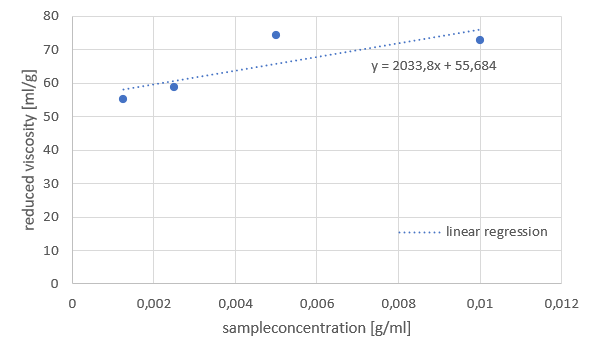
\includegraphics[scale = 0.9]{Bilder/reducedaufconc.png}
				\caption{Reduced viscosity $\eta_\text{red}$ plotted against concentration $c$ using a regression line $\eta_\text{red} = \SI{2033.8}{\frac{ml^2}{g^2}} \cdot c + \SI{55.684}{\frac{ml}{g}}$.}
				\label{reducedaufconcplot}
			\end{figure}

		If a concentration of $\SI{0}{\frac{g}{ml}}$ is substituted into the linear equation, only the y-intercept remains, which in itself yields a viscosity 
		number of $[\eta] = \SI{55.684}{\frac{ml}{g}}$.\\

		This quantity is proportional to the viscosity-weighted molecular weight according to Equation \eqref{ViskosiätsnummerundMolekulargewicht}, 
		which, when rearranged in terms of the viscosity-weighted molecular weight, yields 
		
		\begin{equation}
			M_\eta = \sqrt[a]{\frac{[\eta]}{K}} \text{.}
		\end{equation}
		
		Using the literature values of $K = \SI{0.012}{\frac{ml}{g}}$ and $a = 0.71$, this results in a viscosity-weighted 
		molecular weight of 
		
		\begin{equation*}
			M_\eta = \sqrt[0.71]{\frac{\SI{55.684}{\frac{ml}{g}}}{\SI{0.012}{\frac{ml}{g}}}} = 145933.088 \text{.}
		\end{equation*}

		Therefore the viscosity-weighted molecular weight is $\SI{145933.088}{\frac{g}{mol}}$.\\

		
\section{Questions}

		\subsection{Question 1}

			In total it can be stated, all three of the given polymers have different properties.
			Polystyrene is a neutral polymer and behaves like a statisticall tangle in a good solvent, the Staudinger-index
			only is a referencevalue. The polystyrene-lithium is a living anionic polymer with lithium as a counter ion.
			This lithium-ion forms a polar Li-C-bond in polar solvents, these are also called units.
			These units have a direct influence on the Staudinger-Index, so the index gets higher.
			In the last case of the sulfonated polystyrene is a bit more complex. 
			PSS-Na is a polyelectrolyte, therefore the \ch{SO3-} is distributed over the chain. 
			A uniqueness is if this polymer is put in demineralized water the negative charges repel each other.
			Therefore the polymer swells and the tangle gets bigger, the Staudinger-Index gets very high and is the highest from these three examples.


		\subsection{Question 2}

			At a certain concentration point, things like the intramolecular forces, the hydrodynamic interactions and the entanglements cannot longer be ignored.
			This is because at low concentrations the dilution is assumed to be infinite, therefore the polymer molecule is alone and has no ineractions with other molecules.


		\subsection{Question 3}

			The biggest difference between these two viscometers is the third vent pipe at the Ubeholde-viscosimeters.
			This has the effect, that for the Ubeholde-viscometer the  of the sample is almost irrelevant.
			It also helps to get a constant hydrostatic pressure. 
			Therefore the use cases vary alot between those two. The Ostwald-viscometer is used for individual measurements and the Ubeholde-viscometer is used for dialation measurements.


		\subsection{Question 4}

			The Staudinger-Index of the $it$-PMMA is higher because of the regulary ordered groups the molecule is sterically hindered. 
			The $at$-PMMA has a random order, therefore there is less sterically hindrence.
			Another factor is the solvent, because the $it$-PMMA is already more swallen, the effect of the solvant is even stronger. 


		

\printbibliography

\end{document}